\section{Eigenspace Perturbation Methodology} \label{sec:equips_rans_uq}

The balance of computational cost and fidelity provided by Reynolds Averaged Navier-Stokes (RANS) simulations makes it the tool of choice in most engineering CFD applications. Reynolds averaging starts with the decomposition of the chaotic velocity field ($ u_i$) into its mean ($\overline{u_i}$) and fluctuating ($u_i'$) velocity components such that $u_i = \overline{u_i} + u_i'$. Here $i$ denotes a coordinate direction, $i=1, 2, 3$. This allows for the ensemble-averaging of the Navier-Stokes equations \cite{pope_2000} which leads to a closure problem due to the resulting non-linear $\overline{u_i'u_j'}$ term that has to be modeled. This term is also known as the Reynolds stress tensor, $R_{ij}$.

Turbulence models are concerned with predicting the behavior of the Reynolds stress tensor throughout a flow field of interest, without any a priori high-fidelity data, in a computationally tractable manner. To this end, these models often make simplifying assumptions about the tensor that can inject significant uncertainties into their predictions. For example, a popular assumption that is employed in numerous turbulence models is the Boussinesq approximation (also known as the linear eddy viscosity hypothesis). It assumes that $R_{ij}$ can be defined by a combination of the mean rate of strain ($S_{ij}$), an eddy viscosity ($\nu_t$), and the turbulent kinetic energy ($k$):
 
 \begin{equation}\label{equ:rst}
     R_{ij} = \nu_t S_{ij} - \frac{2}{3} k \delta_{ij},
 \end{equation}
where $S_{ij} = \left ( \frac{\partial \overline{u_i}}{\partial x_j} + \frac{\partial \overline{u_j}}{\partial x_i} \right )$, $x_i$ is a coordinate direction, and $\delta_{ij}$ is the Kronecker delta. This linear eddy viscosity model purports a simplified proportional relationship between the Reynolds stress tensor and the mean rate of strain tensor. It assumes that the turbulent fluid is an isotropic medium where the direction of Reynolds stresses are always aligned with the mean strain rate. Although reasonable for simple flows without adverse pressure gradients, this assumption can severely limit the flow features that can be predicted by the turbulence model, thus introducing uncertainty into the QoIs predicted by RANS simulations. The shortcomings of the Boussinesq assumption are particularly evident in areas of the operating envelope of an aircraft where separated flows and shock-boundary layer interactions exist. 

To better understand the effects of such an assumption, the eigenspace perturbation methodology was developed by Emory et al. \cite{emory2013modeling} and Mishra et al. \cite{iaccarino_eig_pert}. It aims to quantify model-form uncertainties that arise from the use of turbulence models in RANS simulations by introducing perturbations in the eigenvalues and eigenvectors of the Reynolds stress anisotropy tensors $\left ( b_{ij} \right )$ that are predicted by the models. This methodology does not rely on any higher-fidelity data. To explain the perturbations that are introduced, the stress tensor is decomposed into its anisotropic and deviatoric components as
 
\begin{equation}\label{equ:rst_decomp}
    R_{ij}=2k(b_{ij}+\frac{\delta_{ij}}{3}).
\end{equation}
Here, $k~(=\frac{R_{ii}}{2})$ is the turbulent kinetic energy and $b_{ij}$ is the Reynolds stress anisotropy tensor. The anisotropy tensor can be further decomposed into its eigenvalues and eigenvectors and represented as

\begin{equation}\label{equ:eigendecomposition}
b_{ij}=Q \Lambda Q^T,
\end{equation}
where $\Lambda$ is a diagonal matrix that contains the eigenvalues $\lambda_i \in \mathbb{R}$ \cite{Gerolymos2016AlgebraicPA}, and $Q$ is a matrix where the $i$-th column represents the eigenvector corresponding to $\lambda_i$. The matrices $Q$ and $\Lambda$ are ordered such that $\lambda_{1}\geq\lambda_{2}\geq\lambda_{3}$. To understand the eigenspace perturbations it helps to visualize the Reynolds stress tensor as an ellipsoid, where the axes of the ellipsoid are defined by the eigenvectors, the relative lengths along each of the axes are defined by the corresponding eigenvalues, and the size of the ellipsoid is defined by the turbulent kinetic energy. An example of such an ellipsoid, represented in a coordinate system defined by the eigenvectors of $S_{ij}$, is shown in Figure \ref{fig:pert_vis} \textbf{(d)}. 

The perturbations are designed to exercise the limits of the physical realizability constraints placed on the Reynolds stress tensor \cite{schumann1977realizability,speziale1994realizability,2014realizability}. One way to graphically represent the constraints placed on the anisotropic part of the stress tensor is to use the eigenvalues ($\Lambda$) to project the stress tensor onto an anisotropy-invariant map, which often takes the form of a triangle. The vertices of the triangle represent the one-, two- and three-component limiting states of turbulence (referred to as the $1C$, $2C$, and $3C$ states) and all of the physically realizable states of the stress tensor lie within the triangle. One such representation of an anisotropy-invariant map is the barycentric map \cite{banerjee2007presentation}. This mapping allows the writing of the projection as a convex combination of the limiting states of turbulence: 

\begin{equation}\label{equ:barycentric_mapping}
    \textbf{x} = \textbf{x}_{1C} (\lambda_1 - \lambda_2) + \textbf{x}_{2C} (2\lambda_2 - 2\lambda_3) + \textbf{x}_{3C} (3\lambda_3 + 1), 
\end{equation}
where $\textbf{x}_{1C}$, $\textbf{x}_{2C}$, and $\textbf{x}_{3C}$ are the coordinates of the vertices that represent the one-, two-, and three-component limiting states of turbulence. For example, the stress ellipsoid shown in Figure \ref{fig:pert_vis} \textbf{(d)} would be mapped on to the barycentric map as shown in Figure \ref{fig:pert_vis} \textbf{(a)}.

The eigenvalue perturbations are performed such that the limiting states of turbulence are simulated. This involves perturbing the state of the tensor, sequentially, to each of the vertices of the triangle. The eigenvalues resulting from these perturbations are: 

\begin{equation}\label{equ:eigenvalue_pert}
    \Lambda^*_{1C} = 
    \begin{bmatrix}
    2/3 & 0    & 0 \\
    0   & -1/3 & 0 \\
    0   & 0    & -1/3
    \end{bmatrix},~
    \Lambda^*_{2C} = 
    \begin{bmatrix}
    1/6 & 0   & 0 \\
    0   & 1/6 & 0 \\
    0   & 0   & -1/3
    \end{bmatrix},~
    \Lambda^*_{3C} = 
    \begin{bmatrix}
    0 & 0 & 0 \\
    0 & 0 & 0 \\
    0 & 0 & 0
    \end{bmatrix}.
\end{equation}
where $*$ represents the perturbed state. The eigenvector perturbation involves changing the alignment such that the perturbed state is
\begin{equation}\label{equ:eigenvector_pert}
    Q^* = Qv
\end{equation}
where $v$ is either:
\begin{equation}\label{equ:vmin_vmax}
    v_{max} = 
    \begin{bmatrix}
    1 & 0 & 0 \\
    0 & 1 & 0 \\
    0 & 0 & 1
    \end{bmatrix},~
    v_{min} = 
    \begin{bmatrix}
    0 & 0 & 1 \\
    0 & 1 & 0 \\
    1 & 0 & 0
    \end{bmatrix}.
\end{equation}
Combining the eigendecomposition from Equation \eqref{equ:eigendecomposition}, the eigenvalue perturbations from Equation \eqref{equ:eigenvalue_pert}, and the eigenvector perturbations from Equations (\ref{equ:eigenvector_pert}, \ref{equ:vmin_vmax}), the perturbed anisotropy tensor can be built as
\begin{equation}
    b^*_{ij}=Q^* \Lambda^* Q^{*T}.
\end{equation}

In the case shown in Figure \ref{fig:pert_vis} \textbf{(b)}, the eigenvalues are perturbed to the 1C limiting state. This corresponds to changing the shape of the ellipsoid to be infinitely long in one direction, as shown in Figure \ref{fig:pert_vis} \textbf{(e)}. Consequently, the eigenvector alignment is changed to maximize turbulent kinetic energy production ($v_{max}$). This is represented in Figure \ref{fig:pert_vis} \textbf{(c)} and \textbf{(f)}. The change in alignment of the eigenvector can not be represented in the barycentric map, which is why Figures \ref{fig:pert_vis} \textbf{(c)} and \textbf{(b)} are identical.

\begin{figure}
    \center
    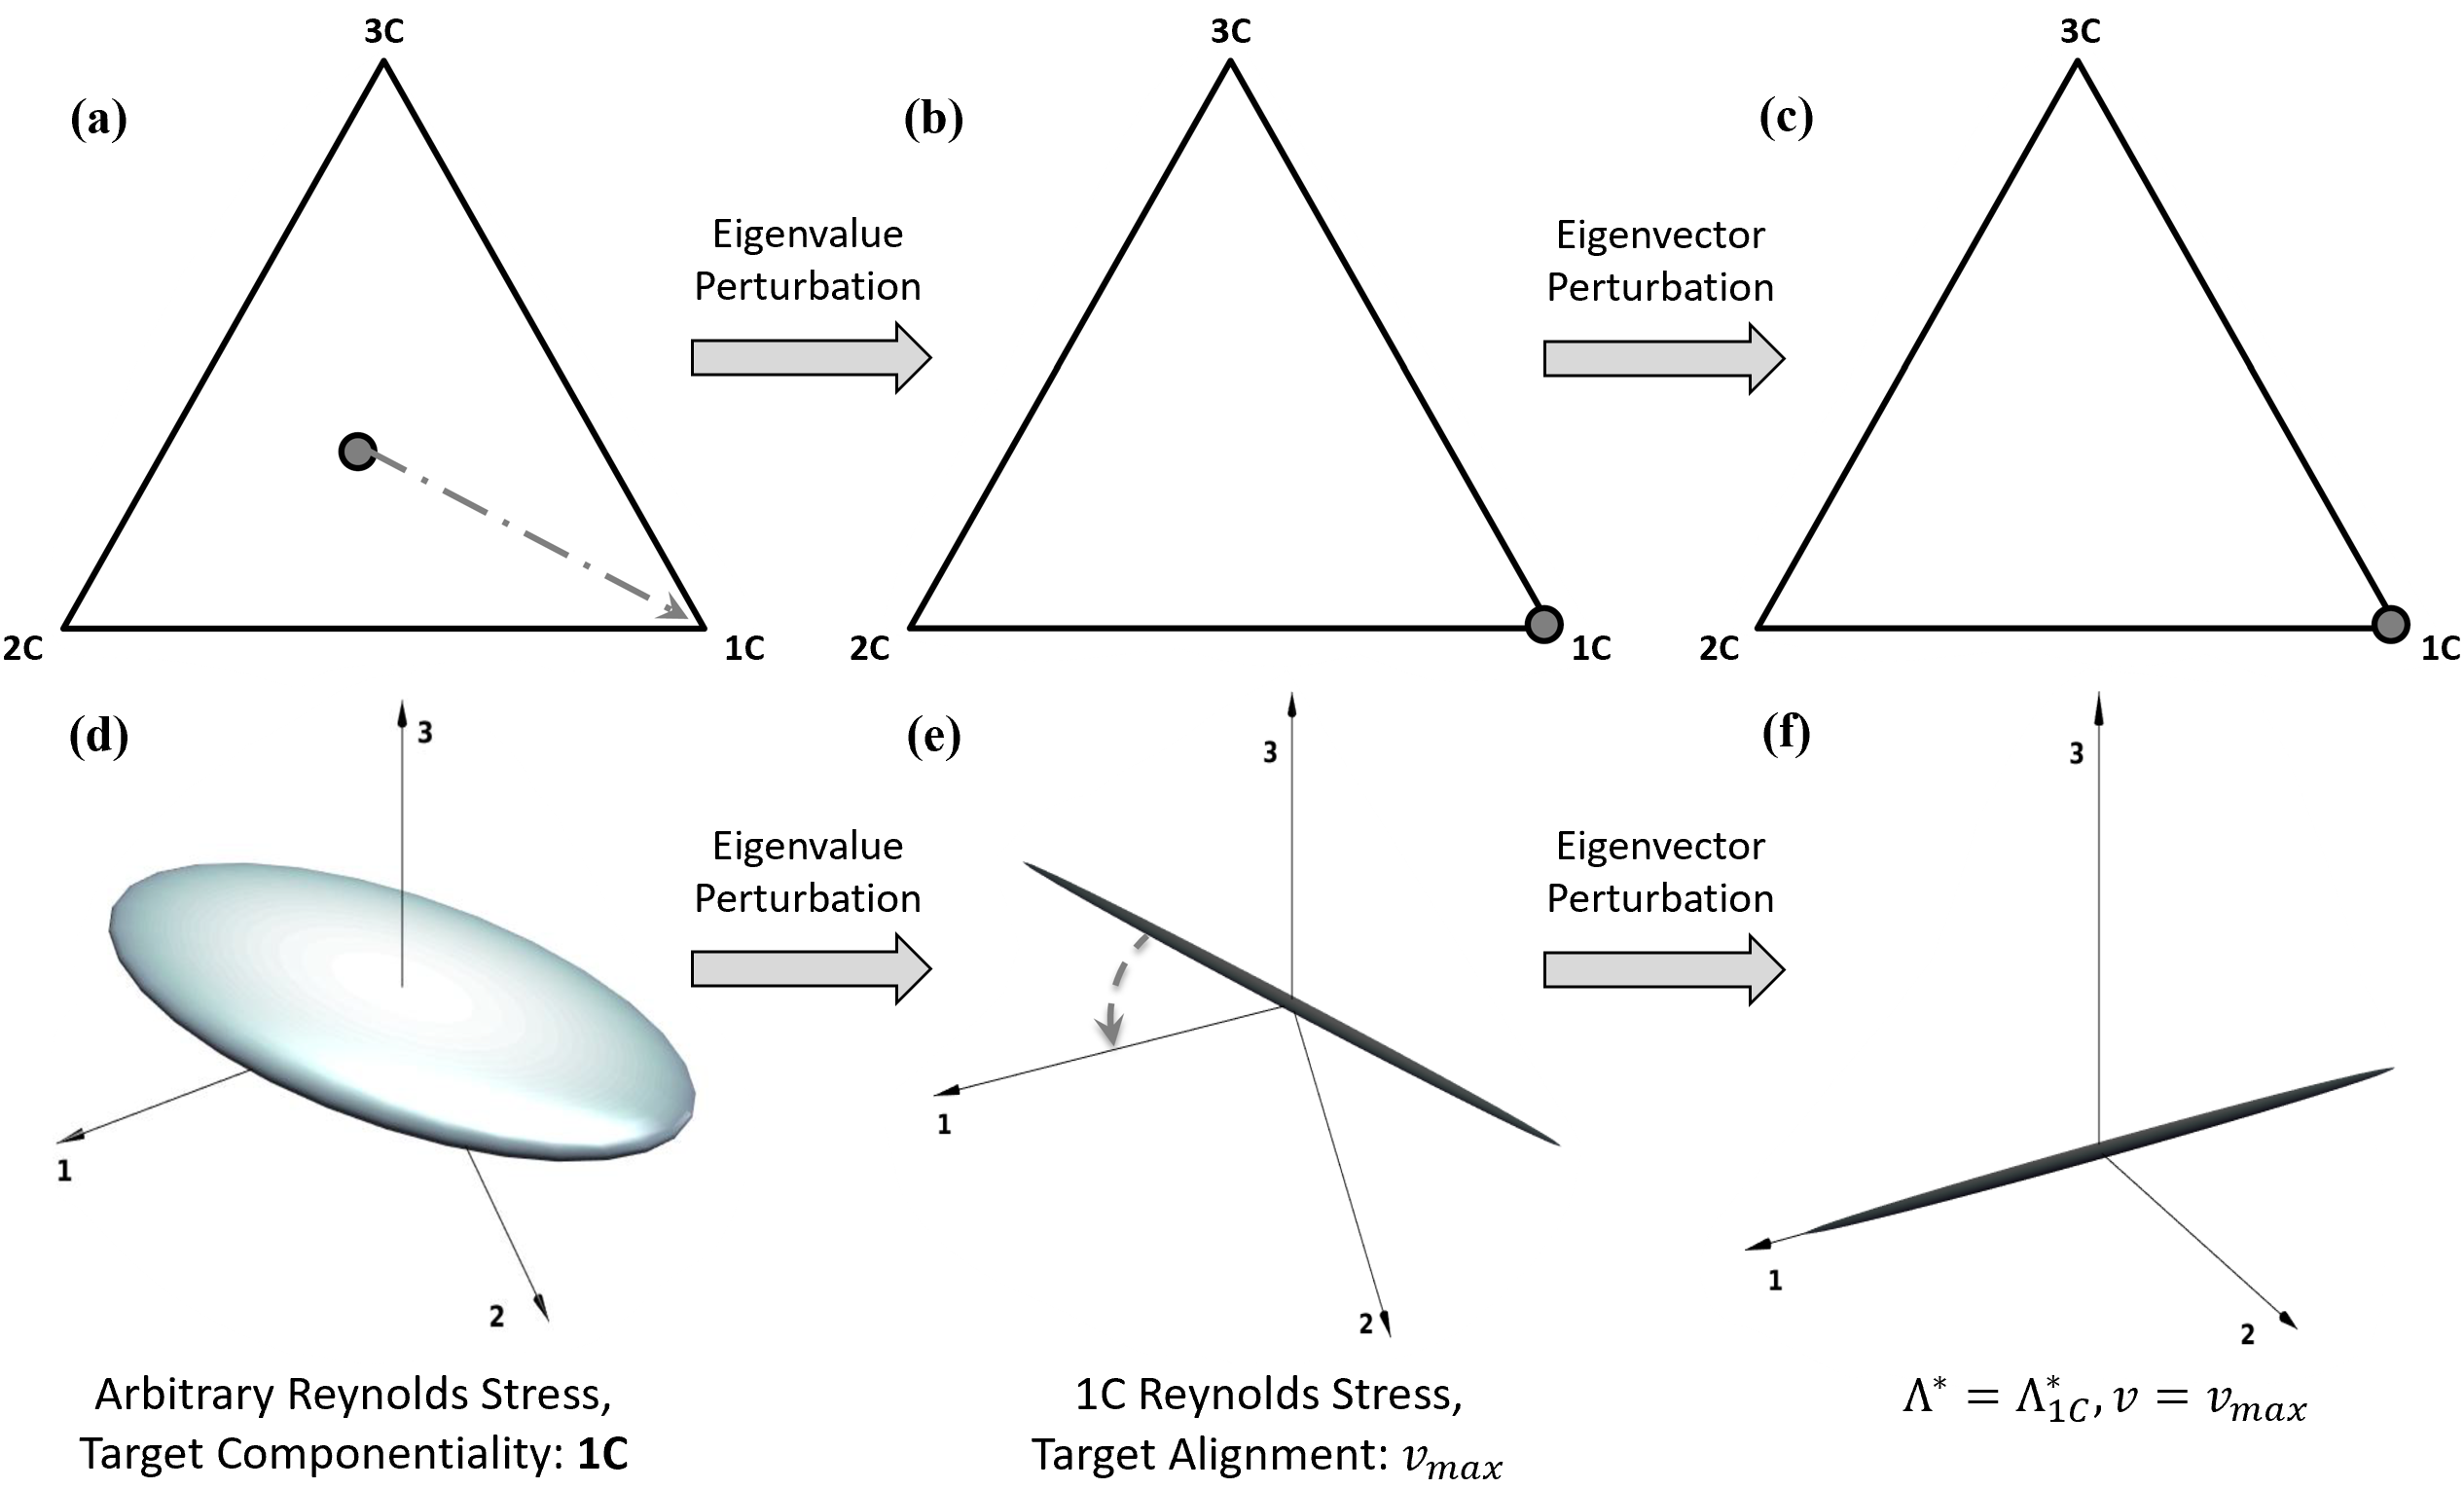
\includegraphics[width=0.95\textwidth]{suthesis/images/eig_pert_1c.png}
    \caption{Schematic outline of Eigenspace perturbations from an arbitrary state of the Reynolds stress. \label{fig:pert_vis}}
\end{figure}

The combinations of 3 eigenvalue perturbations (towards the $1C, 2C$, and $3C$ states) and 2 eigenvector perturbations ($v_{min}$ and $v_{max}$) result in 5 unique sets of perturbations. The resulting Reynolds stress ellipsoid shapes are shown in Figure \ref{fig:all_perts}. This number of perturbations is 5, and not 6, because the $3C$ eigenvalue perturbation results in a rotationally symmetric stress ellipsoid, which means the eigenvector perturbation doesn't change anything. Table \ref{tab:perts} lists the eigenvalue and eigenvector combinations that make up each perturbation. These 5 perturbed states correspondingly require 5 different RANS simulations, in addition to the baseline simulation with the unmodified version of the turbulence model, to provide information about the uncertainty introduced by the turbulence model. For each simulation, the same perturbation is applied uniformly across the entire computational domain, at each pseudo-time step, and the simulation is run to convergence. This results in 5 new realizations of the flow field in addition to the flow field predicted by the unperturbed turbulence model. The maximum and minimum values of any QoI predicted by these 6 (5 perturbed + 1 baseline) simulations create the interval bound for that QoI. These interval bounds are then used in the multi-fidelity framework as uncertainty estimates for CFD simulations. Note that the additional 5 simulations for the perturbed turbulence model can be run simultaneously and, if sufficient computational resources are available, the entire process of RANS UQ can be completed in the same wall-clock time as a typical deterministic RANS simulation.

\begin{table}
\centering
    \def\arraystretch{1.2}
    \begin{tabular}{c|c}
        $\mathbf{\Lambda^*}$ & $\mathbf{Q^*}$ \\\hline
        $\Lambda_{1C}$ & $Qv_{max}$\\
        $\Lambda_{2C}$ & $Qv_{max}$\\
        $\Lambda_{3C}$ & $Qv_{max}$\\
        $\Lambda_{1C}$ & $Qv_{min}$\\
        $\Lambda_{2C}$ & $Qv_{min}$\\
    \end{tabular}
    \caption{Combinations of eigenvalue and eigenvector perturbations that are performed.}
    \label{tab:perts}
\end{table}

An inherent assumption is that the maximum and minimum value of any QoI occurs at the corners of the barycentric triangle, and not somewhere in the interior. In \cite{emory2014visualizing} the bounds were shown to be monotonically increasing as the perturbation magnitude increases. This means that the interval bound is largest at the corner when perturbing along that direction. It is still possible that there could be a different direction of perturbation that would result in larger interval bounds. For example, the largest interval could result from a perturbation towards one of the sides of the barycentric triangle. To exercise the limits of the componentiality of the turbulence field, the perturbations occur towards each vertex of the triangle. 

The theoretical underpinnings of the eigenspace perturbation methodology have been discussed in detail by Mishra and Iaccarino \cite{mishra_perturbations_2019}. They prove that the eigenspace perturbations extend the isotropic eddy viscosity assumption to an anisotropic relation between the mean velocity gradients and the Reynolds stresses. This represents the most general relationship between the mean flow gradients and the Reynolds stresses, $ R_{ij}=\nu_{ijkl}S_{kl}+\mu_{ijkl}W_{kl}$, where $S_{kl}$ and $W_{kl}$ represent the mean rates of strain and rotation respectively. This extension enables the perturbed models to account for the effects of flow separation, secondary flows, highly anisotropic flows, etc. 

The eigenspace perturbation methodology has exhibited substantial success in a variety of engineering applications. This methodology has been successfully applied to the analysis of uncertainty in flows through scramjets \cite{emory2011characterizing}, contoured aircraft nozzles \cite{mishra2019uncertainty,aiaajets, envelopingmodels, alonso2017scalable}, and turbomachinery designs \cite{emory2016uncertainty}. The methodology has been used for the design optimization under uncertainty of turbine cascades \cite{razaaly2019optimization} and in aerospace designs \cite{cook2019optimization}. In civil engineering applications, this methodology has been applied in the design of urban canopies \cite{garcia2014quantifying,ricci2015local}. Owing to the structural similarity between the RANS and LES paradigms, this methodology has been extended and successfully applied for the uncertainty estimation of Large Eddy Simulations and scalar flux models \cite{gorle2013framework} as well.

\begin{figure}
    \centering
    \begin{subfigure}[$2C$ state with $v_{max}$ eigenvector alignment.] {
        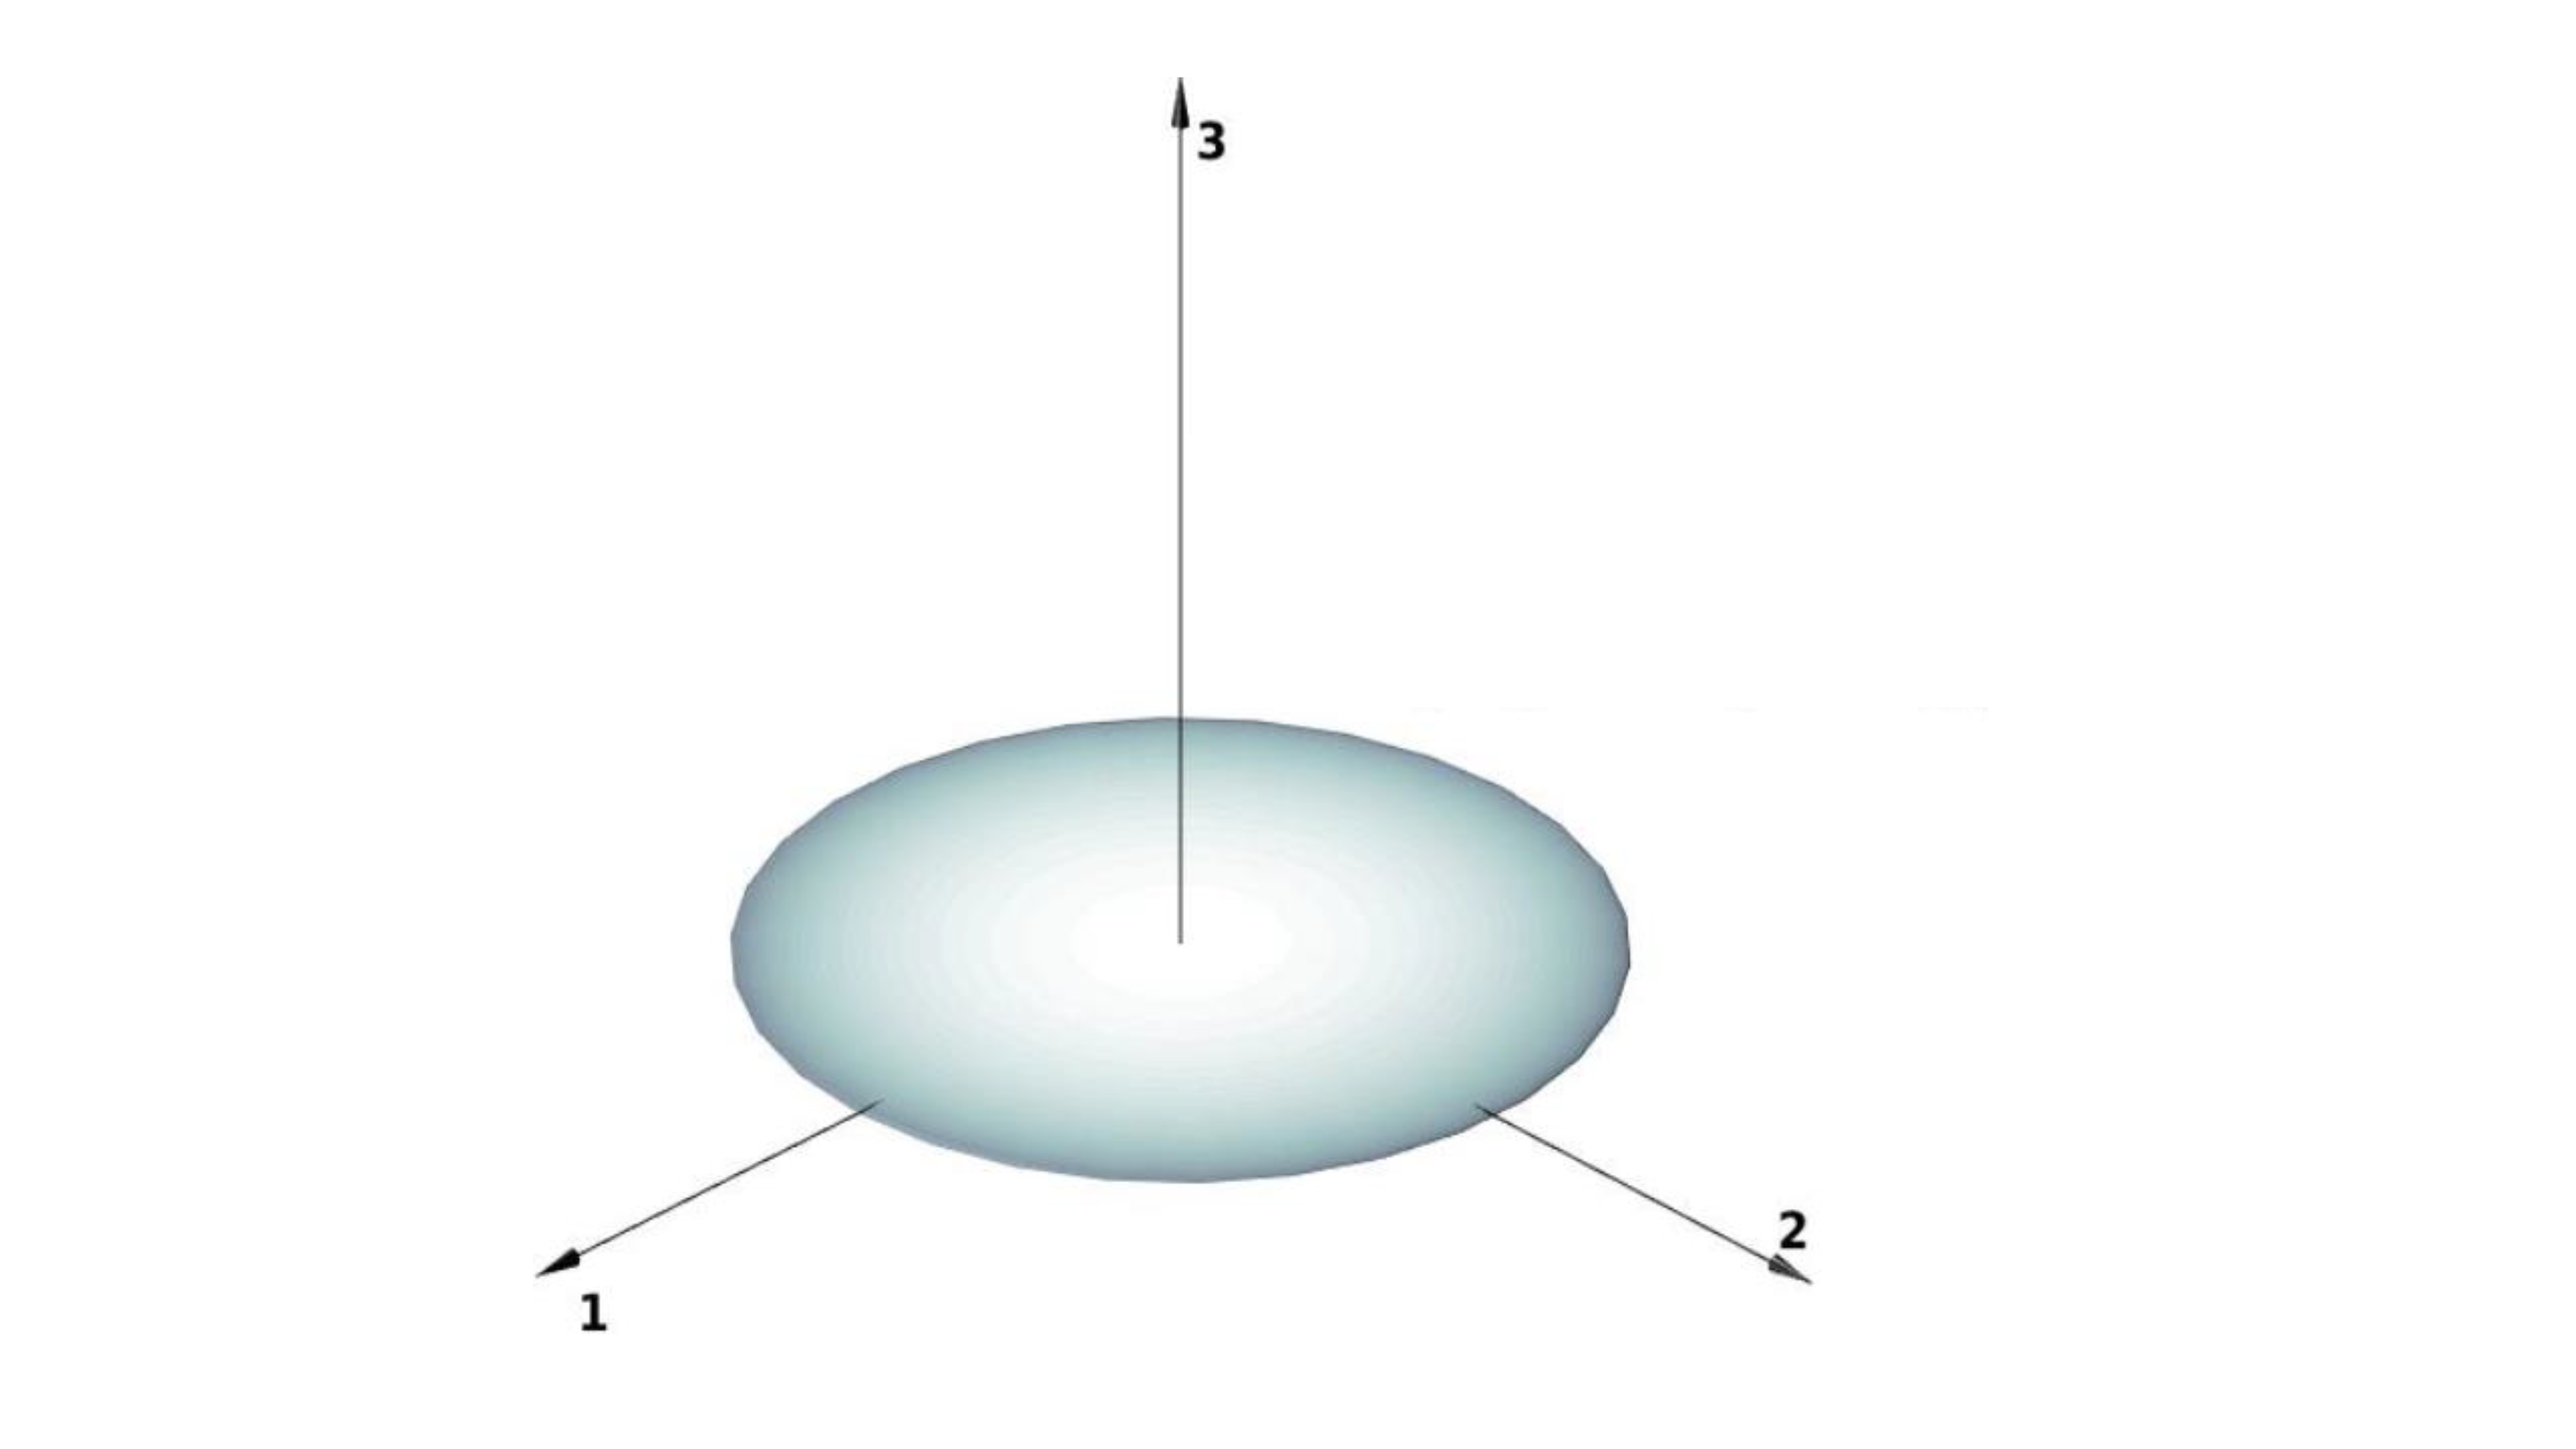
\includegraphics[trim=200 40 280 30, clip, width=0.24\textwidth]{suthesis/images/2c_max.png}
        \label{fig:2c_max}
    }
    \end{subfigure}
    \hspace{10pt}
    \begin{subfigure}[$2C$ state with $v_{min}$ eigenvector alignment.]{
        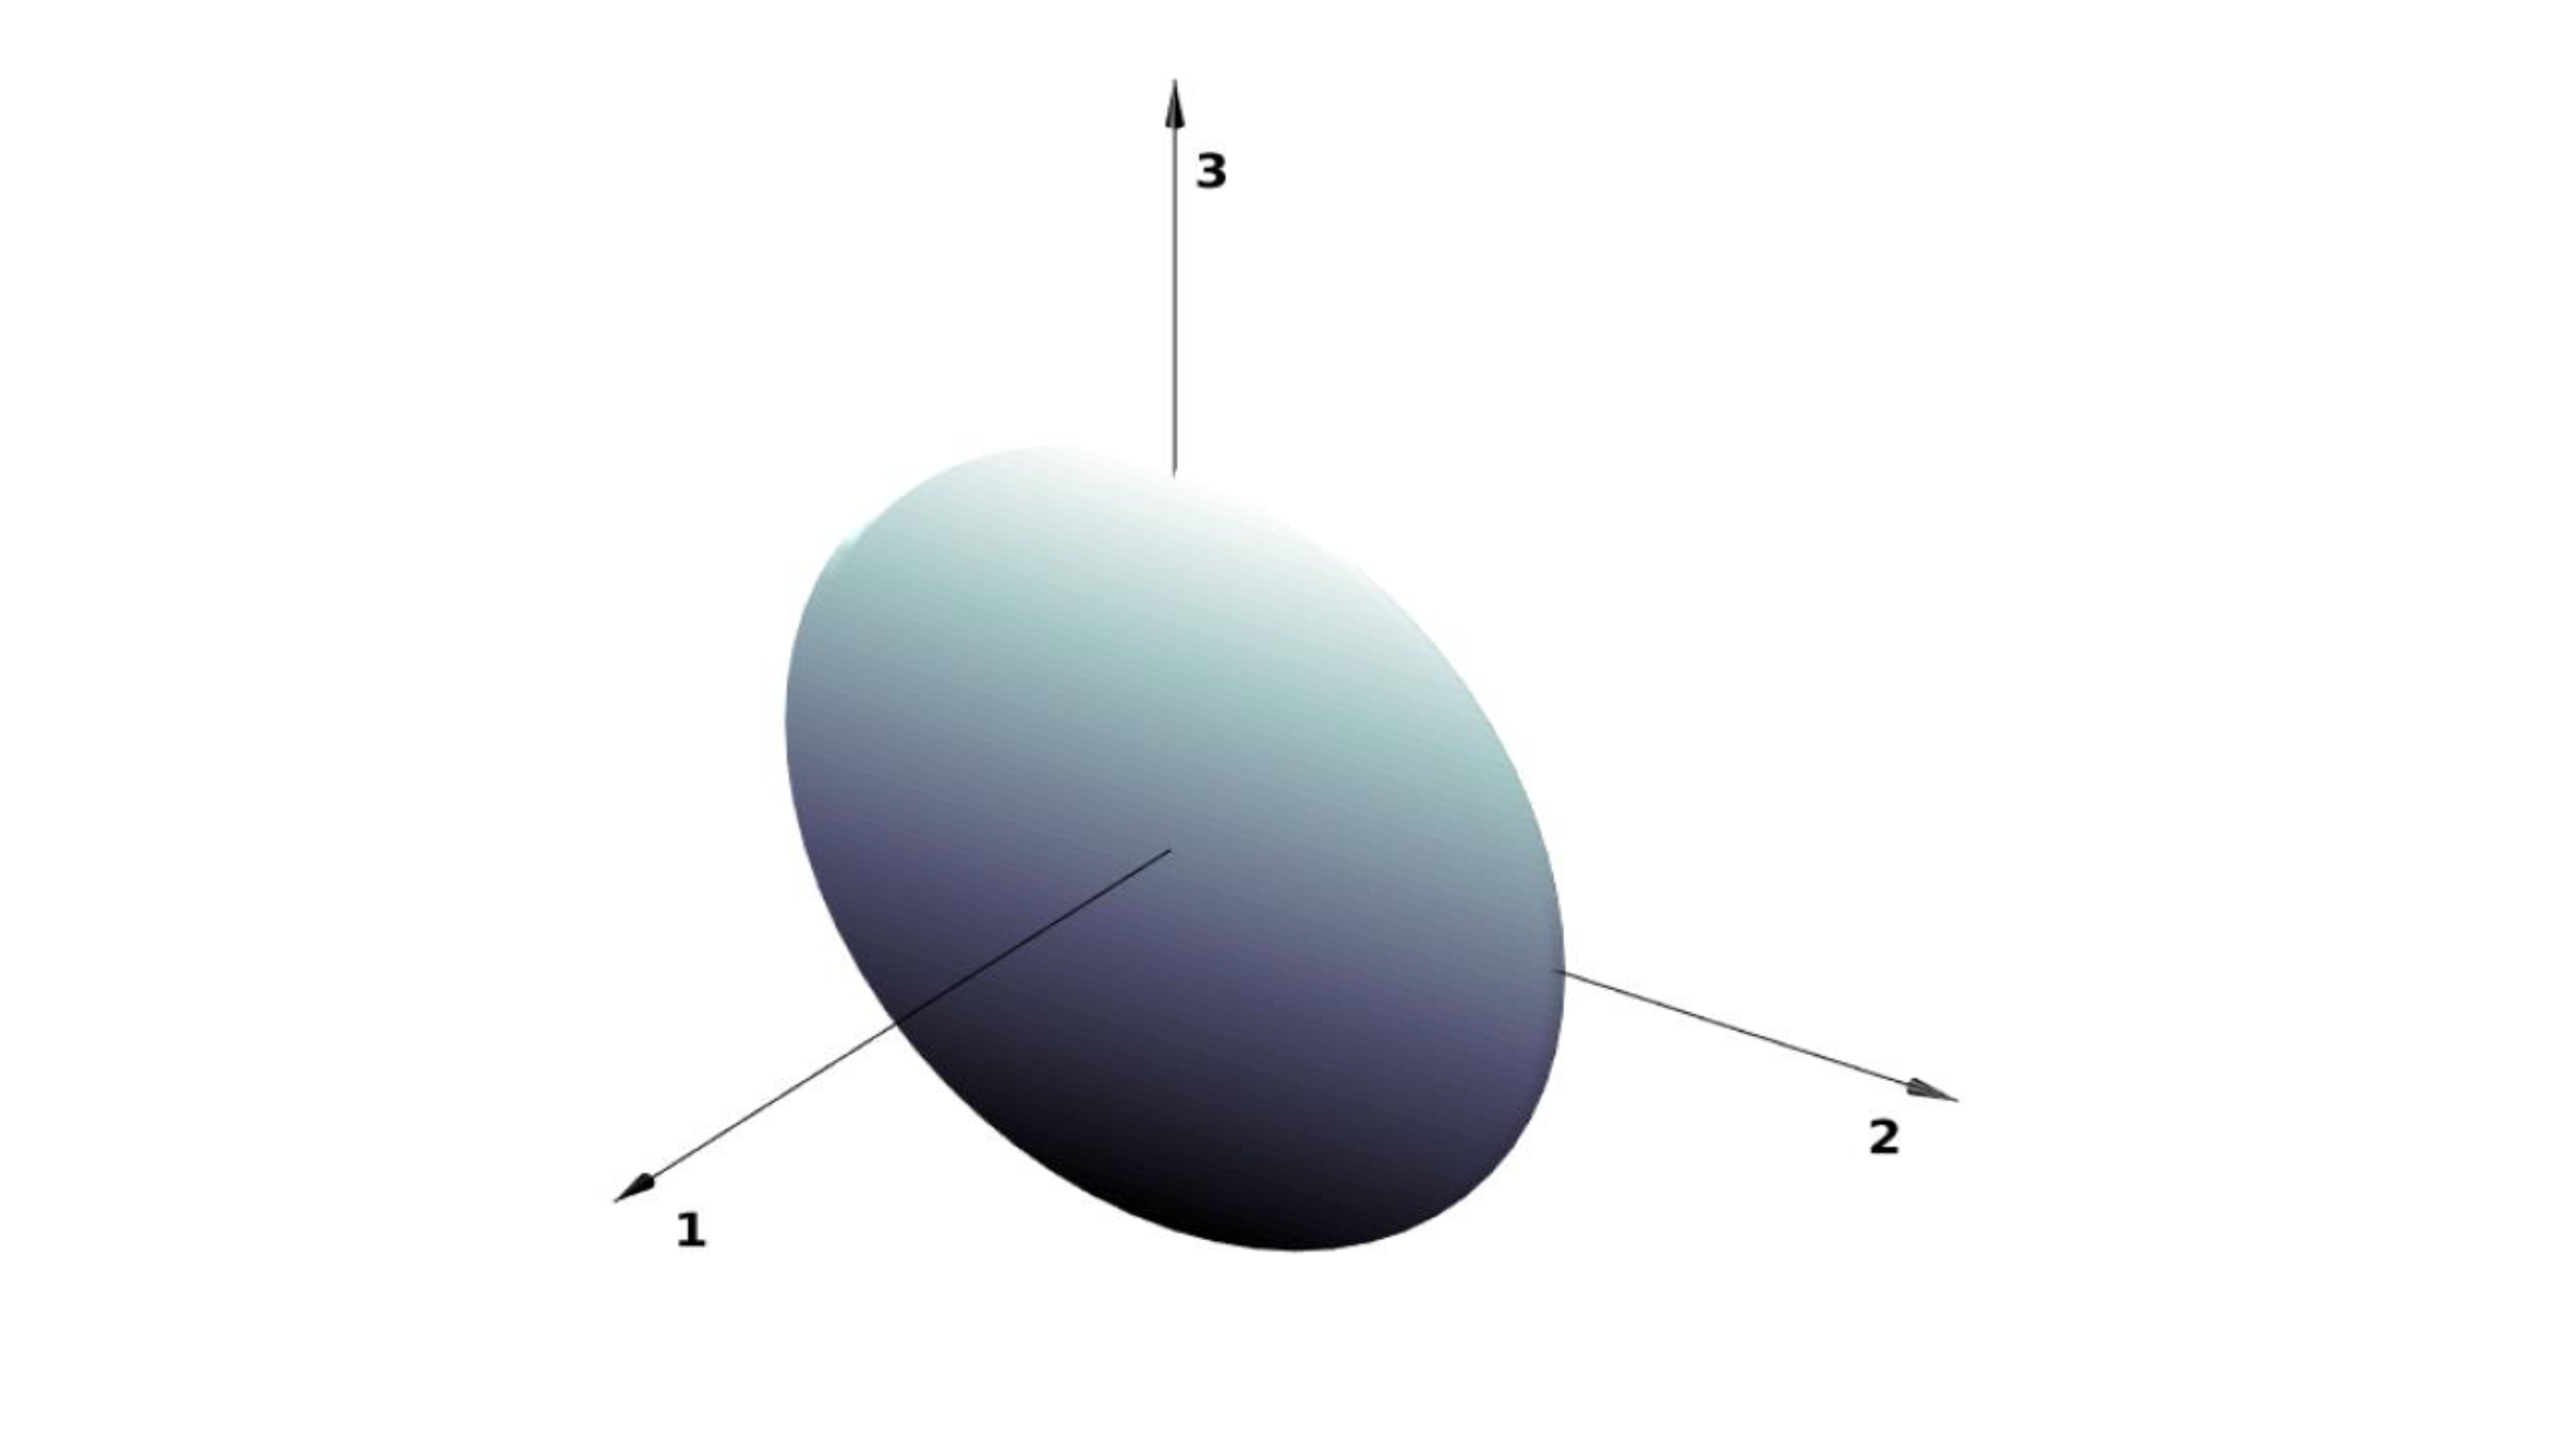
\includegraphics[trim=230 20 230 30, clip, width=0.24\textwidth]{suthesis/images/2c_min.png} 
        \label{fig:2c_min}
    }
    \end{subfigure}
    \hspace{10pt}
    \begin{subfigure}[$3C$ isotropic turbulence state.]{
        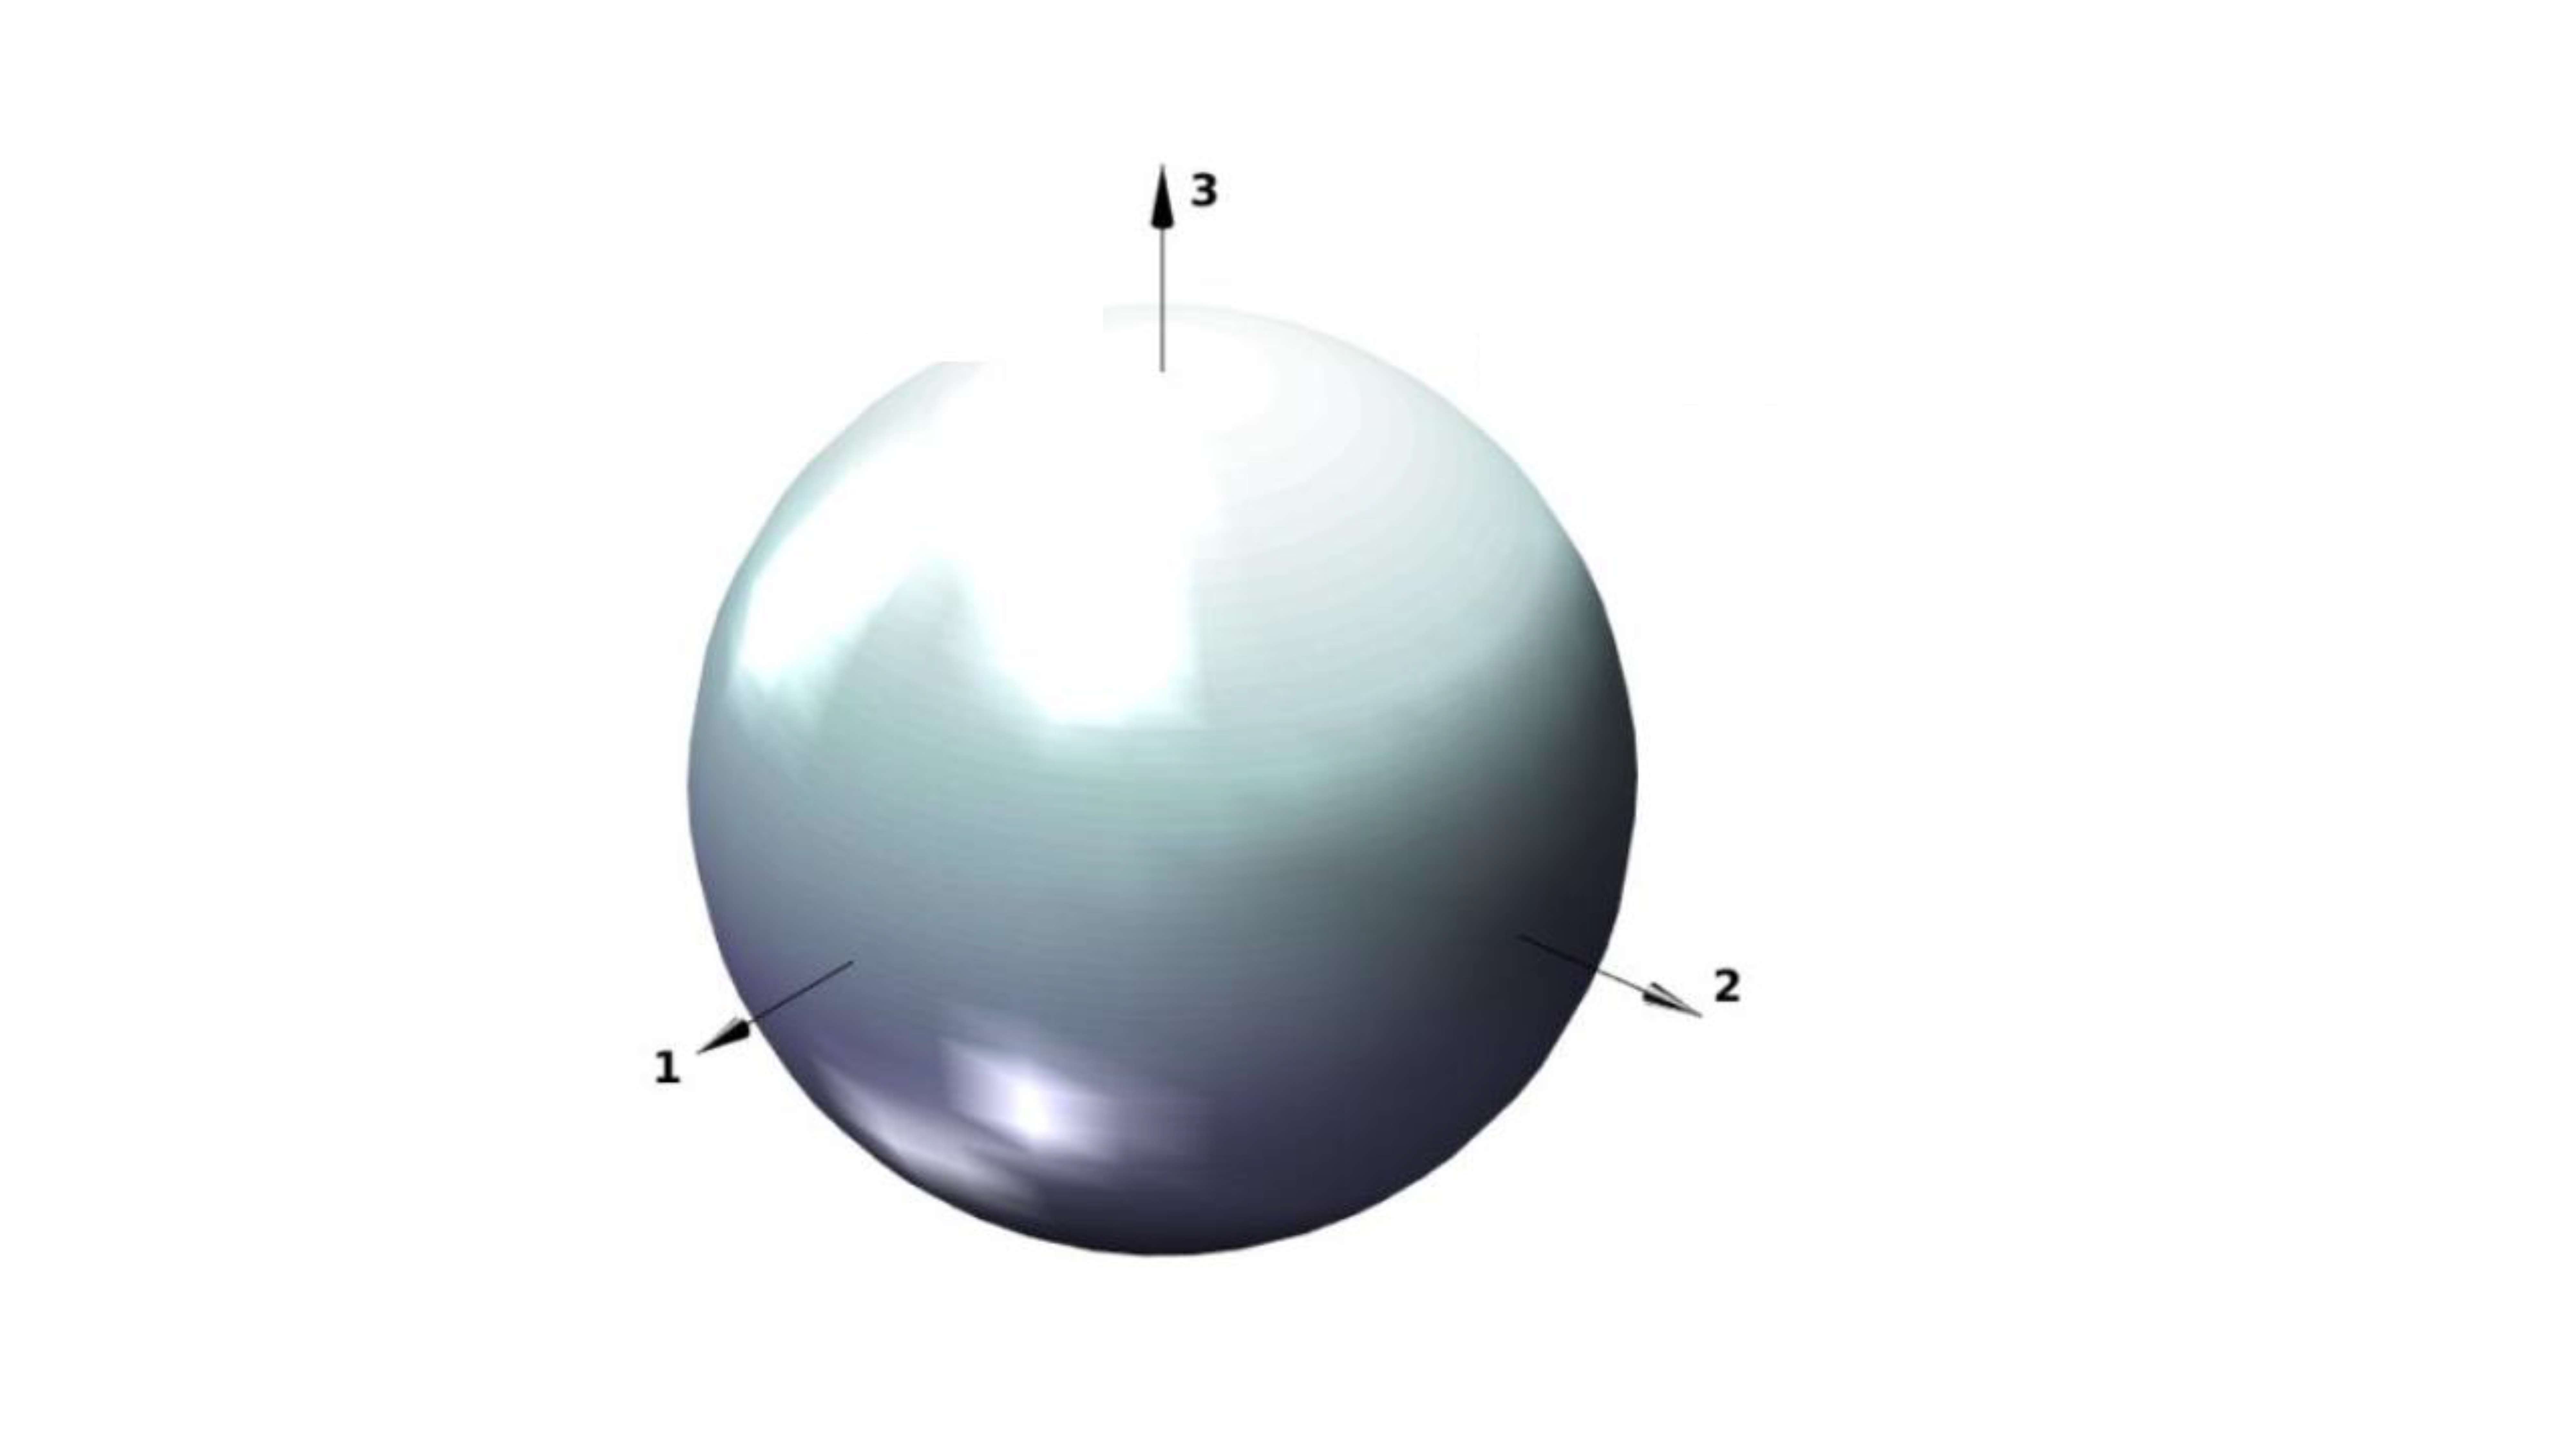
\includegraphics[trim=210 40 280 50, clip, width=0.24\textwidth]{suthesis/images/3c.png} 
        \label{fig:3c}
    }
    \end{subfigure}
    
    \begin{subfigure}[$1C$ state with $v_{max}$ eigenvector alignment.]{
        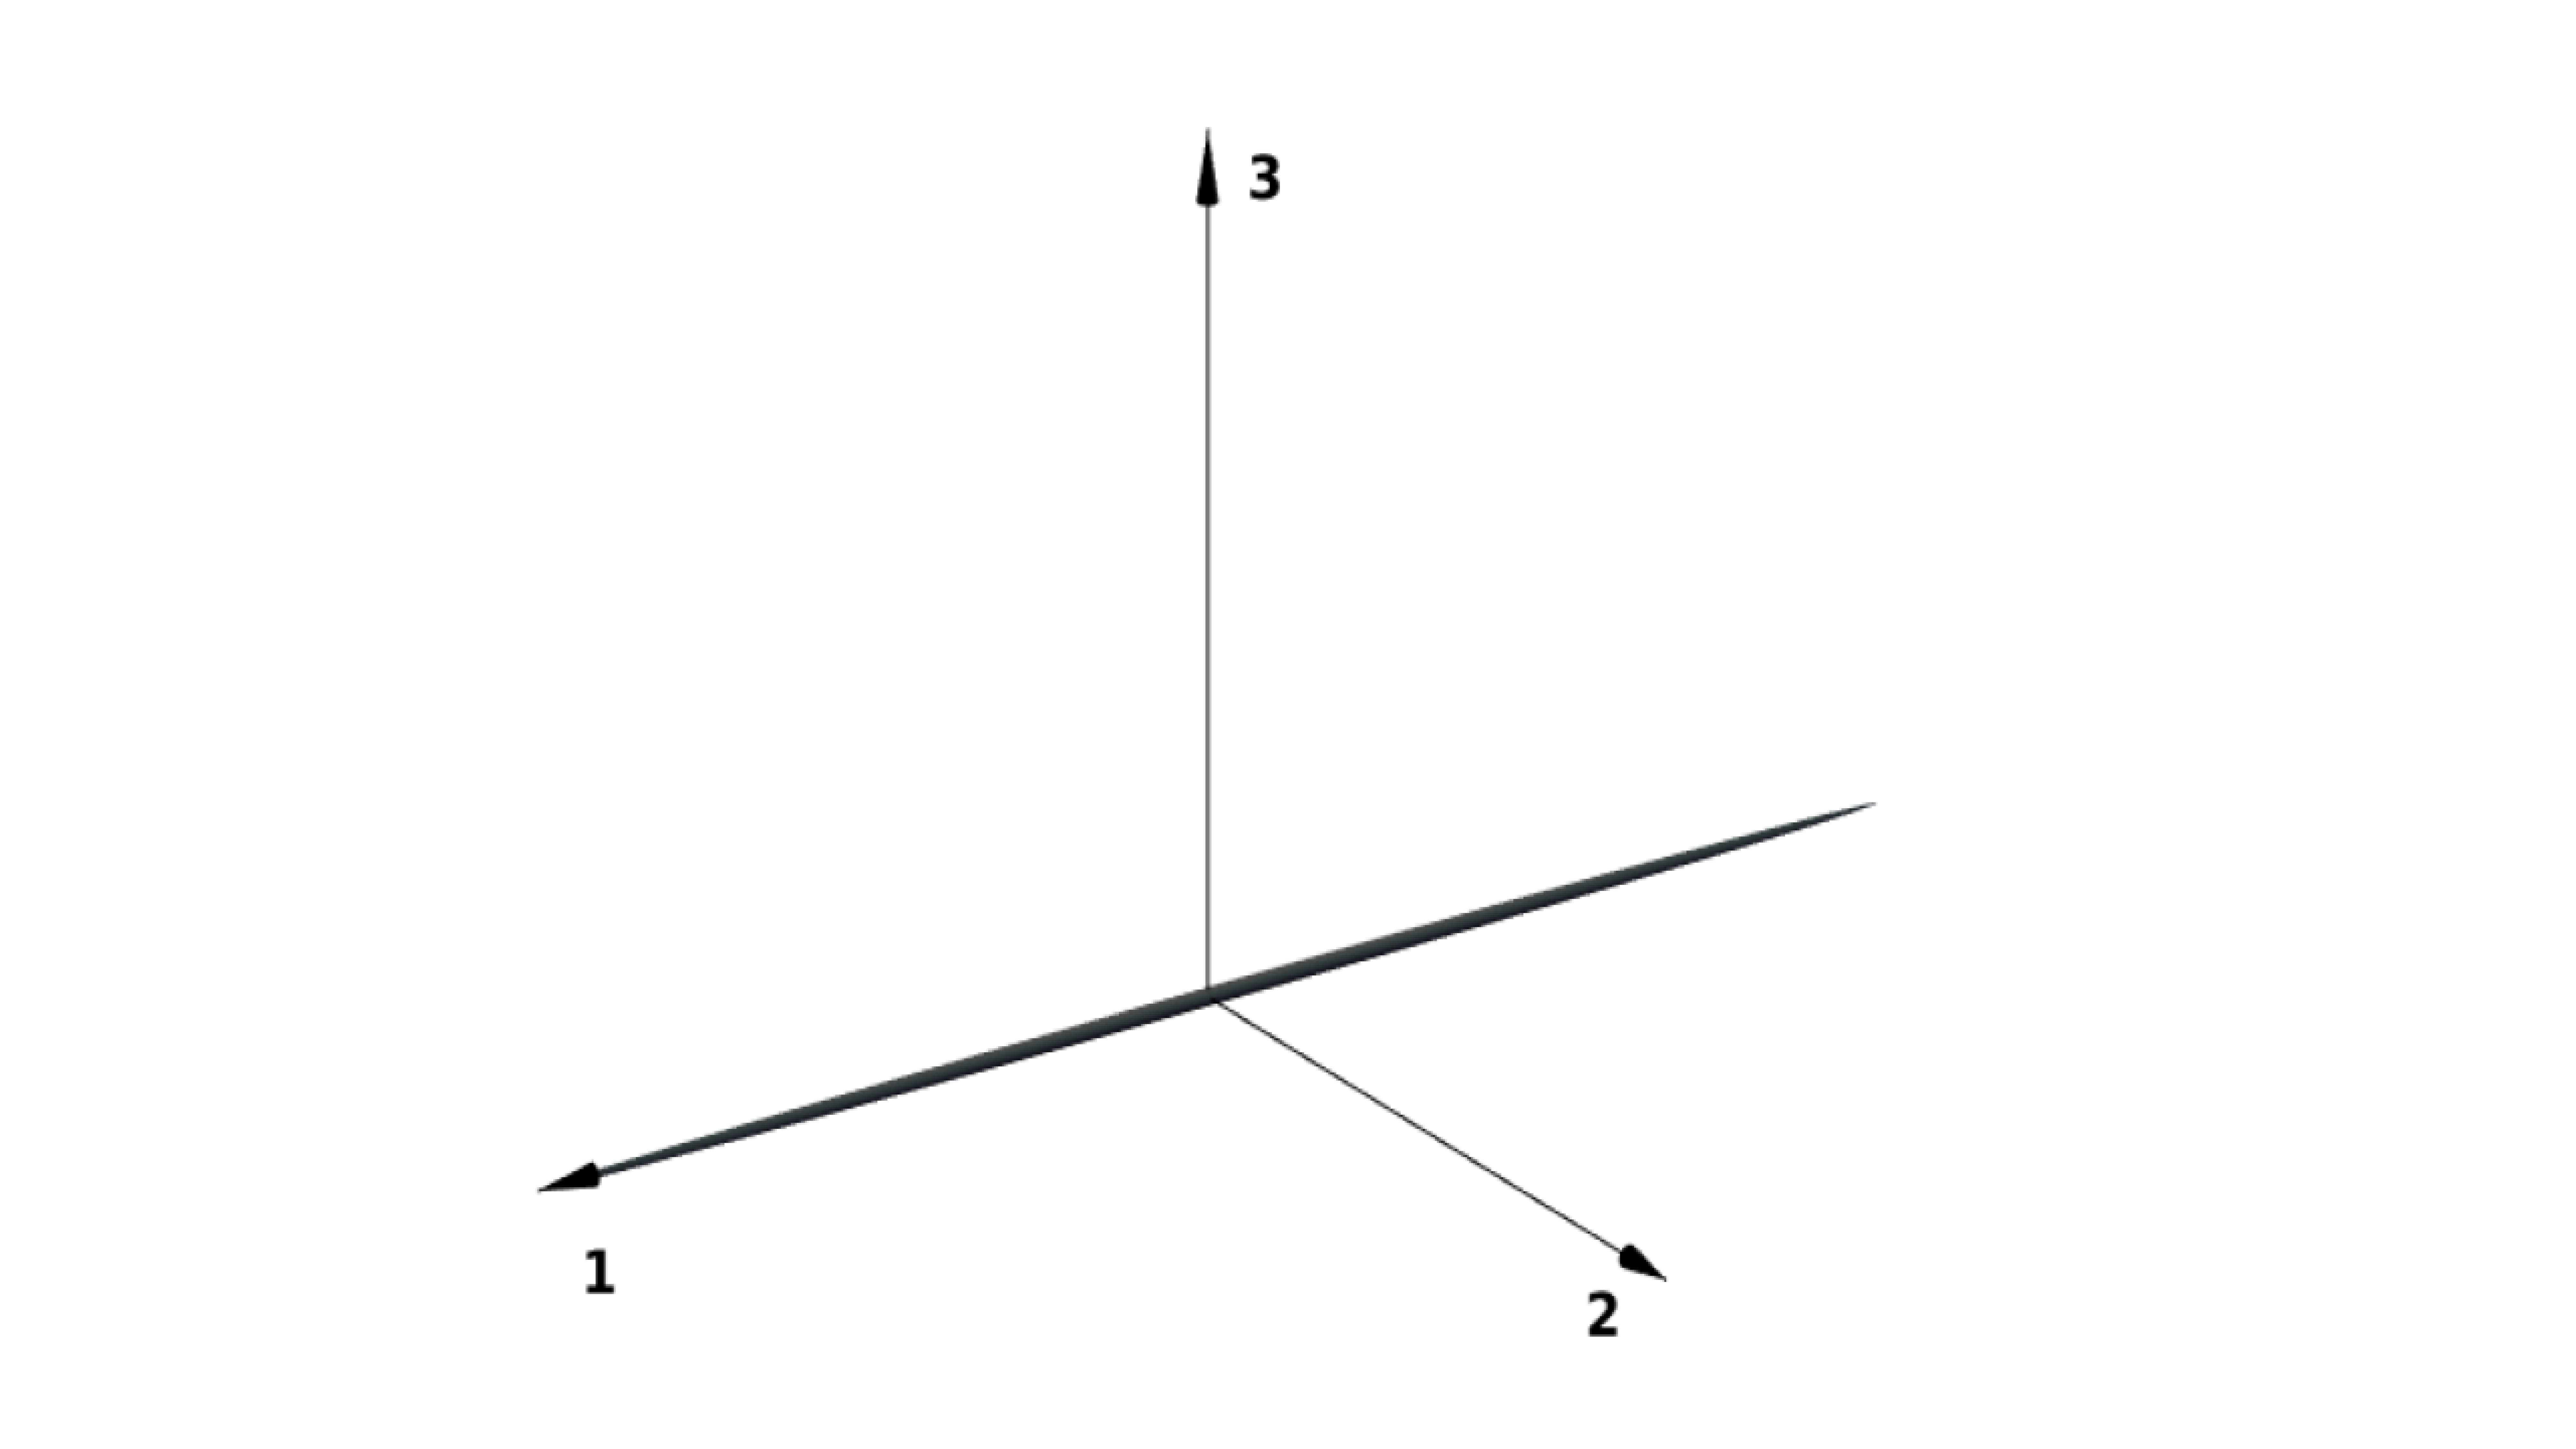
\includegraphics[trim=200 40 300 50, clip, width=0.24\textwidth]{suthesis/images/1c_max.png}
        \label{fig:1c_max}
    }
    \end{subfigure}
    \hspace{10pt}
    \begin{subfigure}[$1C$ state with $v_{min}$ eigenvector alignment.]{
        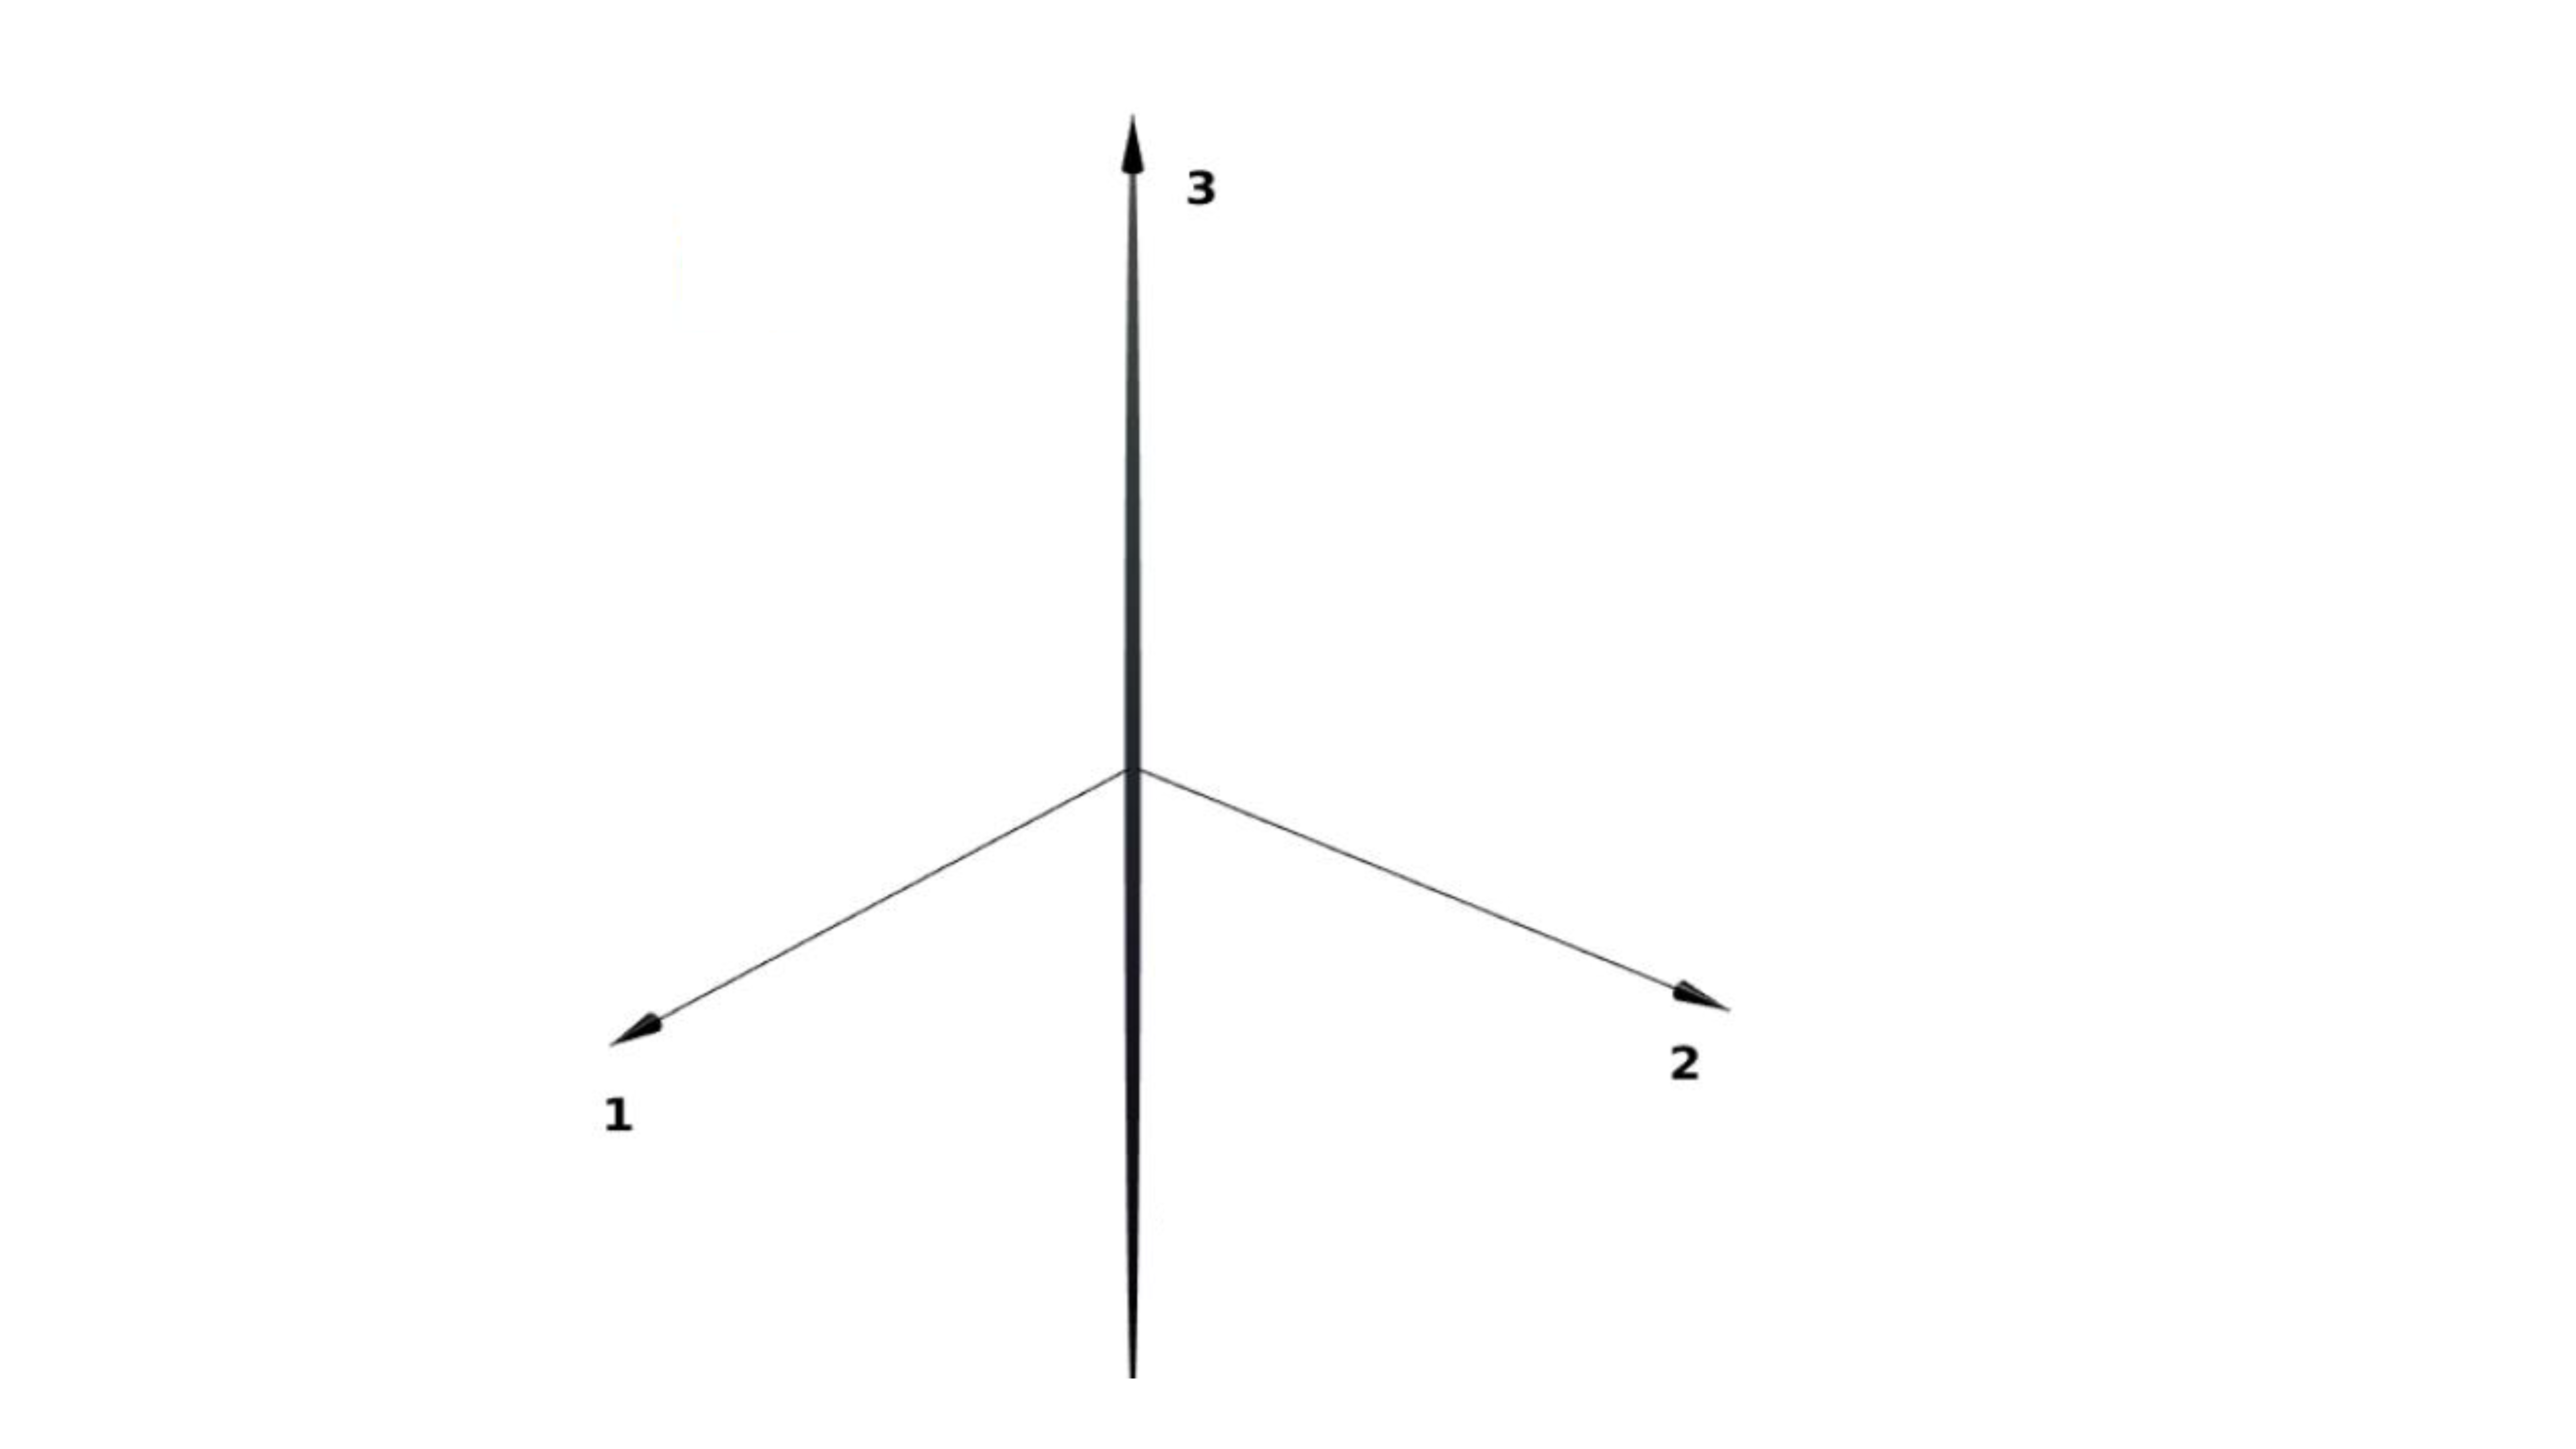
\includegraphics[trim=220 40 300 50, clip, width=000.24\textwidth]{suthesis/images/1c_min.png}
        \label{fig:1c_min}
    }
    \end{subfigure}
    \caption{Graphical visualization of each eigenspace perturbation as Reynolds stress ellipsoids. \label{fig:all_perts}}
\end{figure}

It is important to note that this methodology provides no probability distribution information for the QoIs within these interval bounds and assuming any particular distribution would be inconsistent with the methodology. From Section \ref{sec:mf_modeling}, the multi-fidelity GP requires data to be jointly normally distributed. Consequently, for the purpose of using these interval bounds in the multi-fidelity GP framework, a Gaussian distribution of the QoIs within the bound is assumed. The QoI is given by $y \sim \mathcal{N}(\mu,\sigma^2)$ where $\mu$ is the center of the bound, and $\sigma^2$ is calculated such that $95\%$ of the interval bound predicted by the RANS UQ methodology lies at $2\sigma$ from the mean, $\mu$.